\chapimg{fig/op_pore.png}
\chapterlead{\subhd{After this chapter you can} describe the pores of a soil by their size, shape, origin and connection; derive the capillary law and the Hagen--Poiseuille law and use them to explain why a few large pores carry most of the flow; estimate the saturated conductivity from the geometry of the pores; read a pore-size distribution from a retention curve; and say how tillage, compaction, roots and worms change the geometry.}
\chapter{Pore Geometry and the Architecture of Soil}\label{chap:pore}
\markboth{Pore Geometry and the Architecture of Soil}{Pore Geometry and the Architecture of Soil}
\banner{The space between the grains}
\section{Introduction: why the geometry of the pores matters}
Every property of soil water that this book studies (the retention curve, the field capacity, the conductivity, the response of the soil to irrigation) is a property of the \emph{pores}, not of the grains. The grains give the soil its skeleton, but water and air live in the space between them, and the size, the shape, the number and the connection of the pores decide how much water the soil holds, how strongly it holds it and how fast it moves. Two soils with the same porosity can behave in opposite ways: a sand and a clay may both have a porosity of 0.45, yet the sand drains in minutes and the clay in weeks. The difference is the \emph{geometry}.

\par\noindent This is the first chapter because everything after it rests on it: Chapter~\ref{chap:01} turns the geometry into the retention and conductivity curves, and the later chapters use those curves. The chapter builds the geometry from the beginning. It starts with the classification of pores, derives the two laws that link a pore to the soil water (the capillary law of Young and Laplace, which sets the suction, and the law of Hagen and Poiseuille, which sets the flow), shows how a bundle of pores gives a conductivity, and then adds the complications of real soil: tortuosity, connection, aggregates and macropores. Every formula is followed by an example that can be worked with a pocket calculator.


\begin{figure}[!htbp]\centering\Lfig{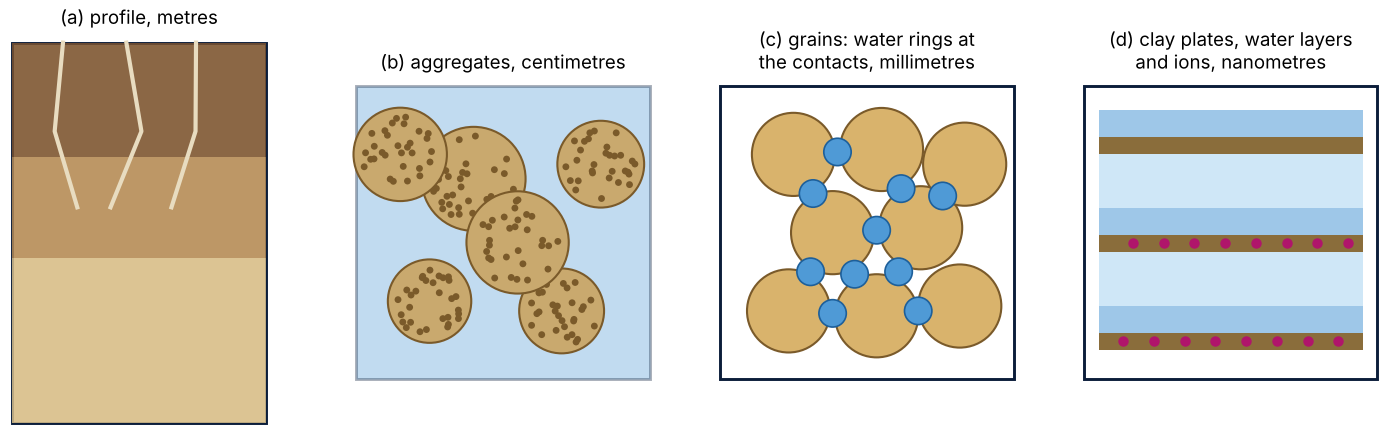
\includegraphics[width=0.92\textwidth]{fig/pg_scales.png}}\caption{The scales of the pore space, from the nanometre to the field. Each class of pore is introduced in this chapter and is tied to the suction at which it empties.}\end{figure}

\subhd{How this chapter is arranged}
The sections follow the order in which the ideas depend on one another:
\begin{exlist}
\item \kw{The quantities} that are used throughout (porosity, water content, suction, surface tension) are defined first.
\item \kw{The pores themselves}: where they come from, how the grains pack, and how the pores are grouped into classes.
\item \kw{The two laws of a single pore}: the Young--Laplace law, which gives the suction at which a pore empties, and the Hagen--Poiseuille law, which gives the flow through it.
\item \kw{Many pores together}: the pore-size distribution, the bundle of capillaries, the share of the flow, tortuosity, connection and the specific surface, which lead to the Kozeny--Carman equation.
\item \kw{Models and real soils}: the retention models, the aggregates, the cracks, the effect of management, and the way the pores are measured.
\end{exlist}

\section{Quantities used in this chapter}\label{sec:quant}
Six quantities are used in every section. They are defined here once, so that the chapter can be read without the next one.
\begin{center}\small\begin{tabular}{@{}p{3.3cm}p{2.0cm}p{2.3cm}p{5.5cm}@{}}\toprule
\hd{Quantity} & \hd{Symbol} & \hd{Unit} & \hd{Meaning and usual value}\\\midrule
Porosity & $\phi$ & m$^3$\,m$^{-3}$ & volume of pores per volume of soil; 0.35 to 0.55\\
Volumetric water content & $\theta$ & m$^3$\,m$^{-3}$ & volume of water per volume of soil; $\theta\le\phi$\\
Suction (matric head) & $h$ & cm of water & the energy per unit weight with which the soil holds water; $\mathrm{pF}=\log_{10}h$\\
Surface tension of water & $\gamma$ & N\,m$^{-1}$ & $0.0728$ at 20\,$^\circ$C\\
Viscosity of water & $\mu$ & Pa\,s & $1.00\times10^{-3}$ at 20\,$^\circ$C\\
Contact angle & $\beta$ & degrees & $0$ for a clean wet mineral wall\\\bottomrule
\end{tabular}\end{center}
\noindent The water content is split into the part held by the pores of each class. The retention curve of the van Genuchten model, $\theta(h)=\theta_r+(\theta_s-\theta_r)[1+(\alpha h)^n]^{-m}$ with $m=1-1/n$, is used in this chapter only to attach numbers to the pore classes; it is derived and discussed in Chapter~\ref{chap:01}.

\section{Pores of a soil: definition and origin}
A \kw{pore} is a void in the soil that is not occupied by solid. Together the pores form the \kw{pore space}, whose volume per unit volume of soil is the porosity $\phi$ (Chapter~\ref{chap:01}). By origin, three groups of pores are distinguished.
\begin{exlist}
\item \kw{Textural pores.} They are the spaces between the individual grains of sand, silt and clay. Their size is set by the size of the grains and by how the grains are packed; they exist in every soil, including a soil without any structure.
\item \kw{Structural pores.} They are the spaces between and inside the aggregates, the crumbs and blocks into which the grains are bound by clay, organic matter and roots. They exist only where there is structure, and they are changed by tillage, compaction, wetting and drying.
\item \kw{Biopores and cracks.} They are made by living roots, by worms and insects (channels of 0.5 to 10 mm), and by the shrinking of a clay as it dries (cracks of 0.1 to 10 mm). They are few, but they are large and continuous, so that they carry a large part of the flow after a heavy rain.
\end{exlist}
\begin{figure}[!htbp]\centering\Lfig{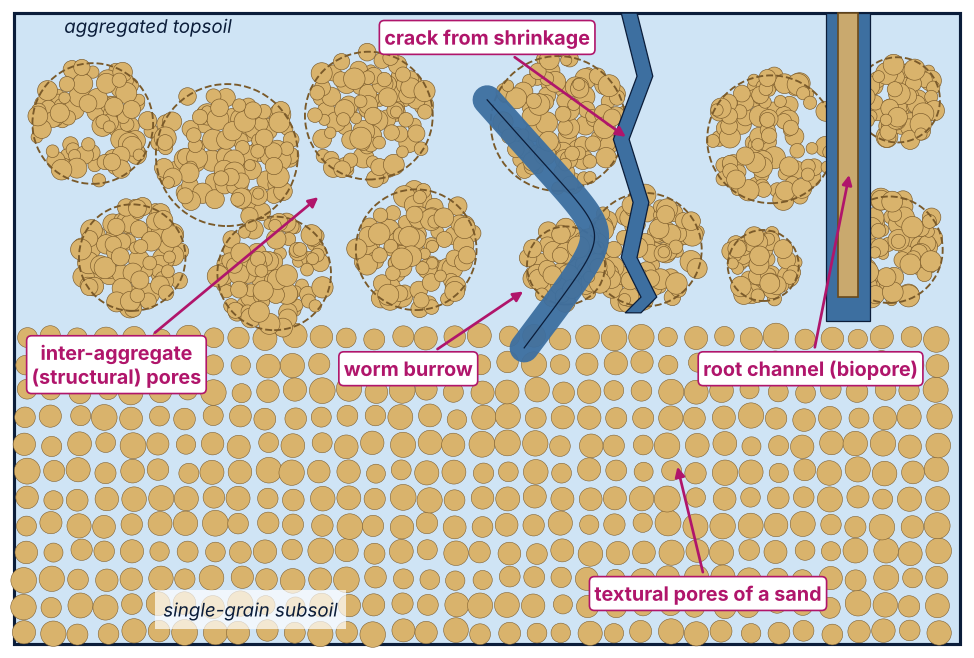
\includegraphics[width=0.94\textwidth]{fig/pg_types.png}}\caption{A section of soil showing the three groups of pores: the textural pores between grains (subsoil), the structural pores between and inside aggregates (topsoil), and the biopores and cracks (worm burrow, root channel and shrinkage crack).}\label{fig:pg-types}\end{figure}

\section{Porosity and the packing of grains}\label{sec:pack}
For grains of one size packed in a regular pattern, the porosity depends only on the arrangement, not on the size of the grains. A \emph{simple cubic} packing of spheres has $\phi=1-\pi/6=0.476$, a \emph{body-centred} packing has $0.320$, and the densest packing, \emph{rhombohedral} (face-centred cubic), has $\phi=1-\pi/(3\sqrt2)=0.260$. A random loose packing of equal spheres has $\phi\approx0.40$ and a random dense packing $\approx0.36$. A real sand has a lower porosity than a packing of equal spheres when the grains have different sizes (the small grains fill the spaces between the large ones), and a clay or an aggregated soil has a higher porosity, because the structure holds the grains apart.
\par\noindent The porosity is found from the densities, $\phi=1-\rho_b/\rho_s$, which divides the pore space into the part filled with water and the part filled with air (Chapter~\ref{chap:01}).
\begin{figure}[!htbp]\centering\Lfig{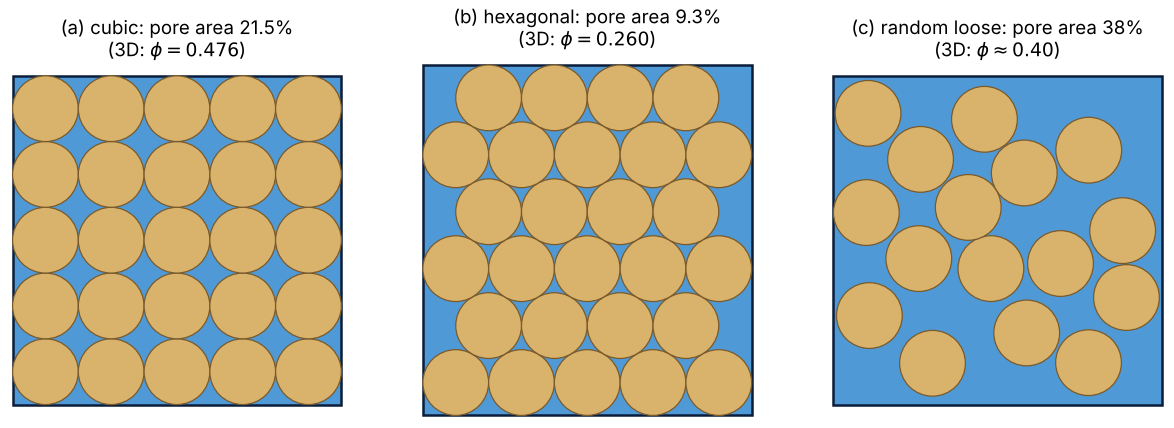
\includegraphics[width=0.92\textwidth]{fig/pg_packing.png}}\caption{Packing of equal spheres: the porosity depends on the arrangement of the grains and not on their size. The pores are the white spaces between the grains.}\label{fig:pg-pack}\end{figure}

\exbox{Porosity from the bulk density}{A topsoil has a dry bulk density $\rho_b=1.30$ g\,cm$^{-3}$ before tillage and $1.50$ g\,cm$^{-3}$ after the passage of a heavy tractor. The particle density is $\rho_s=2.65$ g\,cm$^{-3}$. Find the porosity before and after, and the loss of pore volume.}\sol \givenline{$\rho_b=1.30$ and $1.50$ g\,cm$^{-3}$ ; $\rho_s=2.65$ g\,cm$^{-3}$}
\par\noindent Before: $\phi=1-1.30/2.65=0.509$ \finans. After: $\phi=1-1.50/2.65=0.434$ \finans. The loss is $0.509-0.434=0.075$ m$^3$\,m$^{-3}$, that is $7.5$ per cent of the volume of the soil, or $15$ per cent of the pore space. Because a tractor compresses the large pores first (they are the only ones that are mostly air), if the macroporosity before was $0.12$, it is now about $0.12-0.075=0.045$, a loss of more than 60 per cent. A small change of the bulk density is therefore a large change of the macropores.

\banner{Capillarity: the law that links a pore to the suction}\label{ch:pg-cap}
\section{Classification of pores by size}
Because the pore sizes of a soil range over five orders of magnitude (from a few nanometres to several millimetres), the pores are grouped into classes, and each class has a role. The limits are most easily set by the suction at which a pore empties (Section~\ref{sec:cap}).
\begin{center}\small\begin{tabular}{@{}p{3.0cm}p{2.7cm}p{2.5cm}p{4.9cm}@{}}\toprule
\hd{Class} & \hd{Equivalent radius} & \hd{Empties at} & \hd{Function in the soil}\\\midrule
Macropores & $>15\ \mu$m & $h<100$ cm (pF $<2$) & air, roots, fast drainage; carry the flow after rain\\
Mesopores & 15 to 0.09 $\mu$m & pF 2 to 4.2 & store the water that the plants take up (the available water)\\
Micropores & $<0.09\ \mu$m & pF $>4.2$ & hold water tightly; not available to plants; bacteria live here\\\bottomrule
\end{tabular}\end{center}
\noindent \textbf{Notes:} 1. The limits are the ones used in this book: the suction of field capacity (100 cm) and of the permanent wilting point (15\,849 cm). Other authors use other limits (for example, 30 and 0.2 $\mu$m in diameter), but all are applications of the same law. 2. A \emph{functional} classification is also used: \kw{transmission pores} (larger than about 50 $\mu$m, which carry water and air quickly), \kw{storage pores} (0.5 to 50 $\mu$m, which hold water for the crop) and \kw{residual pores} (below 0.5 $\mu$m, which hold water that cannot be used).

\begin{figure}[!htbp]\centering\Lfig{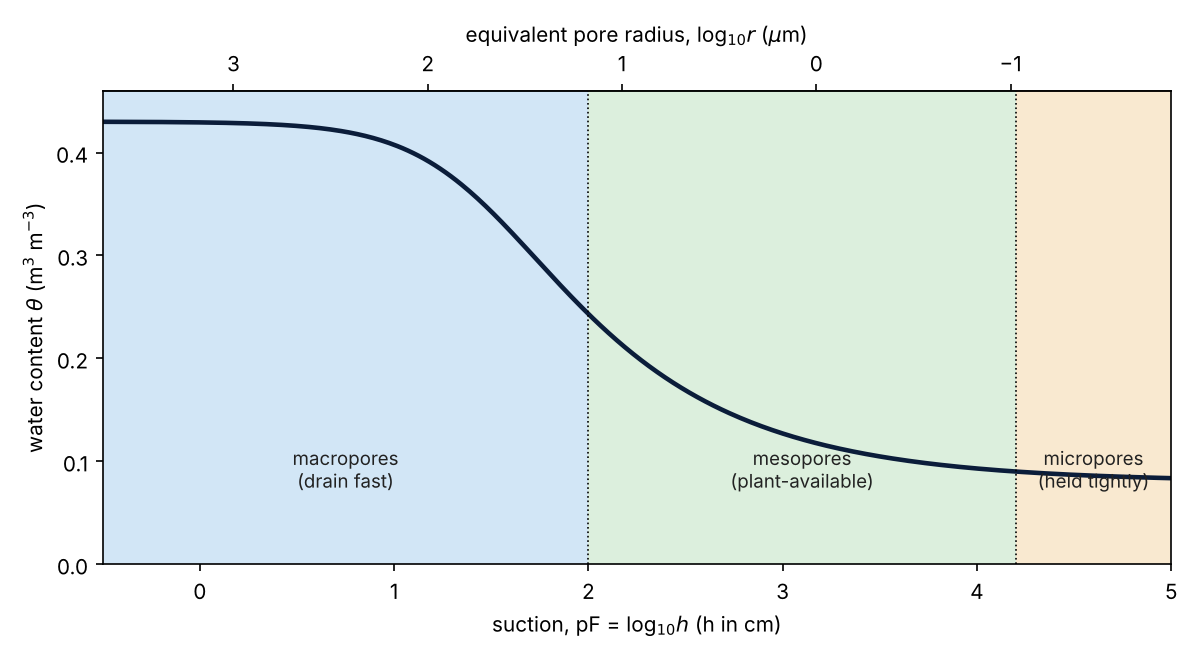
\includegraphics[width=0.92\textwidth]{fig/pore_domains.png}}\caption{The pore classes on the retention curve of the loam of Chapter~\ref{chap:01} ($\alpha=0.036$ cm$^{-1}$, $n=1.56$, $\theta_s=0.43$, $\theta_r=0.08$). The suction on the lower axis corresponds to the pore radius of the upper axis through Equation~(\ref{eq:pg-cap}).}\label{fig:pg-dom}\end{figure}

\begin{figure}[!htbp]\centering\Lfig{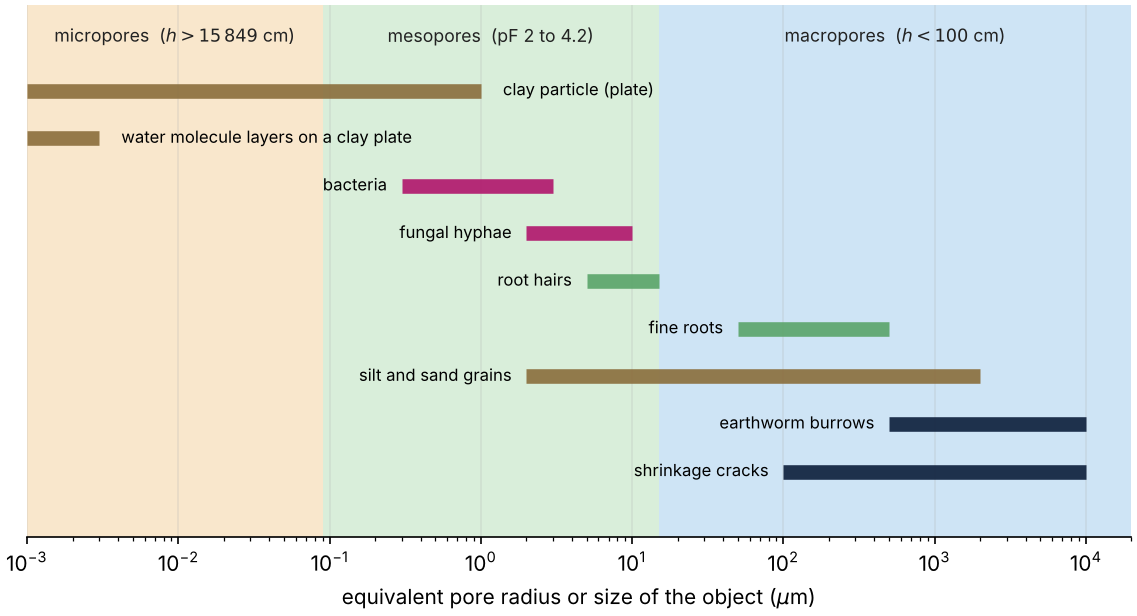
\includegraphics[width=0.92\textwidth]{fig/pg_ladder.png}}\caption{The ladder of the pore classes: the equivalent radius of each class, the suction at which it empties (from Equation~\ref{eq:pg-cap}) and the role it plays in the soil.}\end{figure}

\section{The Young--Laplace law: derivation}\label{sec:cap}
Water in a narrow pore is pulled upward by the attraction between the water and the wall (adhesion) and held together by the surface tension $\gamma$. Consider a cylindrical tube of radius $r$ that is wetted by water with a contact angle $\beta$ between the water surface and the wall. The upward force acts along the line of contact, of length $2\pi r$, with the vertical component $\gamma\cos\beta$:
\[F_{up}=2\pi r\,\gamma\cos\beta .\]
At equilibrium the weight of the raised column, of height $h$, is $F_{down}=\pi r^2h\,\rho_w g$. Equating the two forces gives the height of the rise, which is the suction that the pore exerts:
\begin{equation}\label{eq:pg-cap}\boxed{h=\frac{2\gamma\cos\beta}{\rho_w\,g\,r}\ \approx\ \frac{0.149}{r}\ \ (h\text{ and }r\text{ in cm}),}\end{equation}
where $h$ is the capillary rise or suction (m), $\gamma=0.0728$ N\,m$^{-1}$ the surface tension of water at 20 $^\circ$C, $\beta\approx0$ for water on clean mineral surfaces, $\rho_w=998$ kg\,m$^{-3}$, $g=9.81$ m\,s$^{-2}$ and $r$ the radius of the pore (m). The law was found by Young and by Laplace in 1805; it says that the narrower the pore, the higher the water is held and the larger the suction at which the pore empties.
\par\noindent \textbf{Notes:} 1. The pressure difference across the curved surface is $\Delta p=2\gamma\cos\beta/r$; the suction in length of water is $h=\Delta p/(\rho_wg)$. 2. The soil pore is not a cylinder, so $r$ is an \emph{equivalent} radius: the radius of the cylinder that would empty at the same suction. 3. A pore empties when the suction reaches the value of its \emph{narrowest part} (the neck), not its widest, which is the physical origin of hysteresis (Chapter~\ref{chap:01}). 4. If the water does not wet the wall completely ($\beta>0$, as in a soil that is water-repellent after a fire or after heavy organic matter), the rise is smaller and, for $\beta>90^\circ$, water is pushed out of the pore instead.

\begin{figure}[!htbp]\centering\Lfig{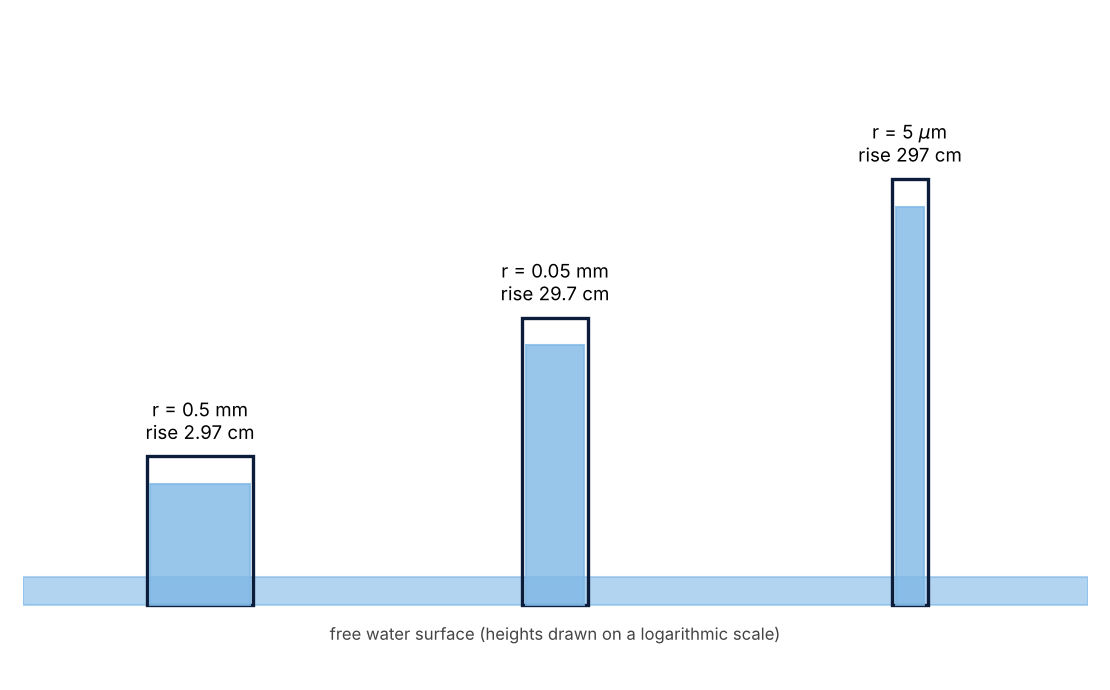
\includegraphics[width=0.84\textwidth]{fig/pore_rise.png}}\caption{Capillary rise in three tubes. The height is inversely proportional to the radius (Equation~\ref{eq:pg-cap}), so that a tube ten times narrower holds water ten times higher.}\end{figure}

\begin{figure}[!htbp]\centering\Lfig{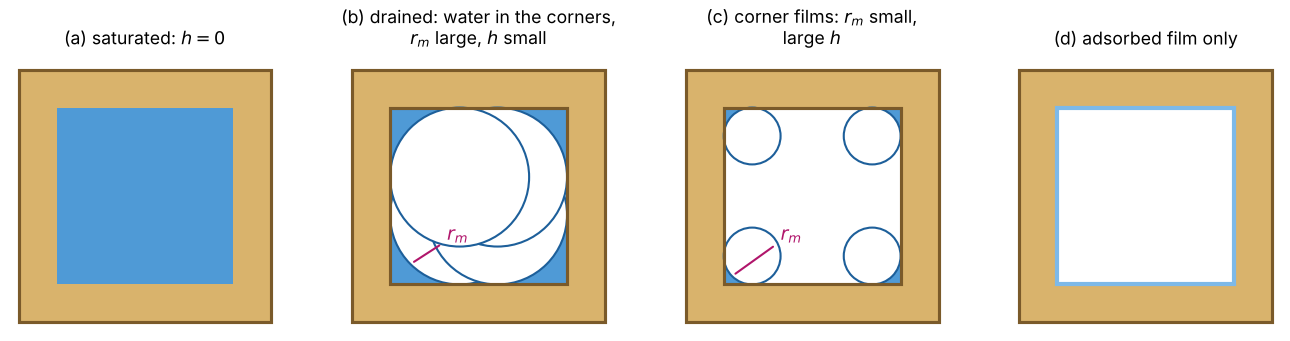
\includegraphics[width=0.92\textwidth]{fig/pg_corner.png}}\caption{Drying of an angular pore: the centre of the pore empties first, while the water stays in the corners, where the meniscus has the smallest radius $r_m$. This is why a drying soil keeps a little conductivity long after its large pores are empty.}\end{figure}

\begin{center}\small\begin{tabular}{@{}rrrrl@{}}\toprule
\hd{$h$ (cm)} & \hd{pF} & \hd{$r$ ($\mu$m)} & \hd{$2r$ ($\mu$m)} & \hd{Meaning}\\\midrule
1 & 0.0 & 1490 & 2980 & the pores of a gravel or a coarse crack\\
10 & 1.0 & 149 & 298 & a coarse sand\\
100 & 2.0 & 14.9 & 29.8 & the limit of field capacity\\
300 & 2.5 & 4.97 & 9.93 & the trigger of a sensor\\
1000 & 3.0 & 1.49 & 2.98 & a clay at moderate suction\\
15\,849 & 4.2 & 0.094 & 0.188 & the permanent wilting point\\\bottomrule
\end{tabular}\end{center}

\exbox{The suction of a pore, and the pore of a suction}{(a) What is the suction at which a pore of radius 20 $\mu$m empties? (b) What is the radius of the largest pore that is still full of water in a soil at a suction of 300 cm?}\sol \givenline{(a) $r=20\ \mu\mathrm m=2\times10^{-3}$ cm ; (b) $h=300$ cm}
\par\noindent \textbf{(a)} From Equation~(\ref{eq:pg-cap}), $h=0.149/(2\times10^{-3})=74.5$ cm \finans, that is pF $1.87$: such a pore drains before the field capacity of 100 cm is reached, so it belongs to the macropores.
\par\noindent \textbf{(b)} $r=0.149/300=4.97\times10^{-4}$ cm $=4.97\ \mu$m \finans. At a trigger of 300 cm, all the pores wider than 5 $\mu$m are empty, and the water is held in the finer pores: the amount of water that is held depends on how much of the pore volume is below this size, which is read from the retention curve.

\section{The pore-size distribution from the retention curve}\label{sec:psd}
Because each suction corresponds to one pore radius, the retention curve is a measurement of the pore-size distribution. If $\theta(h)$ is the water content at suction $h$, then $\theta_s-\theta(h)$ is the volume of the pores wider than $r(h)$, and the volume of the pores whose radius lies between $r$ and $r+\mathrm dr$ follows by differentiation. It is usual to plot the density per decade of suction (per unit of pF),
\begin{equation}\label{eq:pg-psd}\boxed{f(\mathrm{pF})=-\frac{\mathrm d\theta}{\mathrm d\,\mathrm{pF}}=-\ln10\;h\,\frac{\mathrm d\theta}{\mathrm dh},}\end{equation}
where $f$ is the pore volume per unit volume of soil per decade of pore radius. For the van Genuchten curve (Chapter~\ref{chap:01}) the derivative can be written in closed form,
\[-\frac{\mathrm d\theta}{\mathrm dh}=(\theta_s-\theta_r)\,m\,n\,\alpha\,(\alpha h)^{n-1}\bigl[1+(\alpha h)^n\bigr]^{-m-1},\]
which has a single maximum, at the \kw{dominant pore size}. The pore-size curves of the ten soils are shown in Figure~\ref{fig:a19_7}: the coarse soils have a narrow, tall peak at small pF, and the clays a wide, low one at large pF.

\exbox{The volume of each pore class in the loam}{For the loam with $\alpha=0.036$ cm$^{-1}$, $n=1.56$, $\theta_s=0.43$ and $\theta_r=0.08$, the retention curve gives $\theta(100)=0.243$ and $\theta(15\,849)=0.090$. Find the volumes of the macropores, the mesopores and the micropores.}\sol \givenline{$\theta_s=0.43$ ; $\theta(100)=0.243$ ; $\theta(15\,849)=0.090$}
\par\noindent The macropores are the pores that are empty at field capacity: $\theta_s-\theta(100)=0.430-0.243=0.187$ \finans. The mesopores are emptied between field capacity and wilting: $\theta(100)-\theta(15\,849)=0.243-0.090=0.153$ \finans, which is $153$ mm of available water per metre of soil, the value of Chapter~\ref{chap:01}. The micropores hold $\theta(15\,849)=0.090$ \finans. The three add to $0.430$, the porosity, so the classes are complete. Almost half of the pore volume (43 per cent) is macropore space in this loam.

\begin{figure}[!htbp]\centering\Lfig{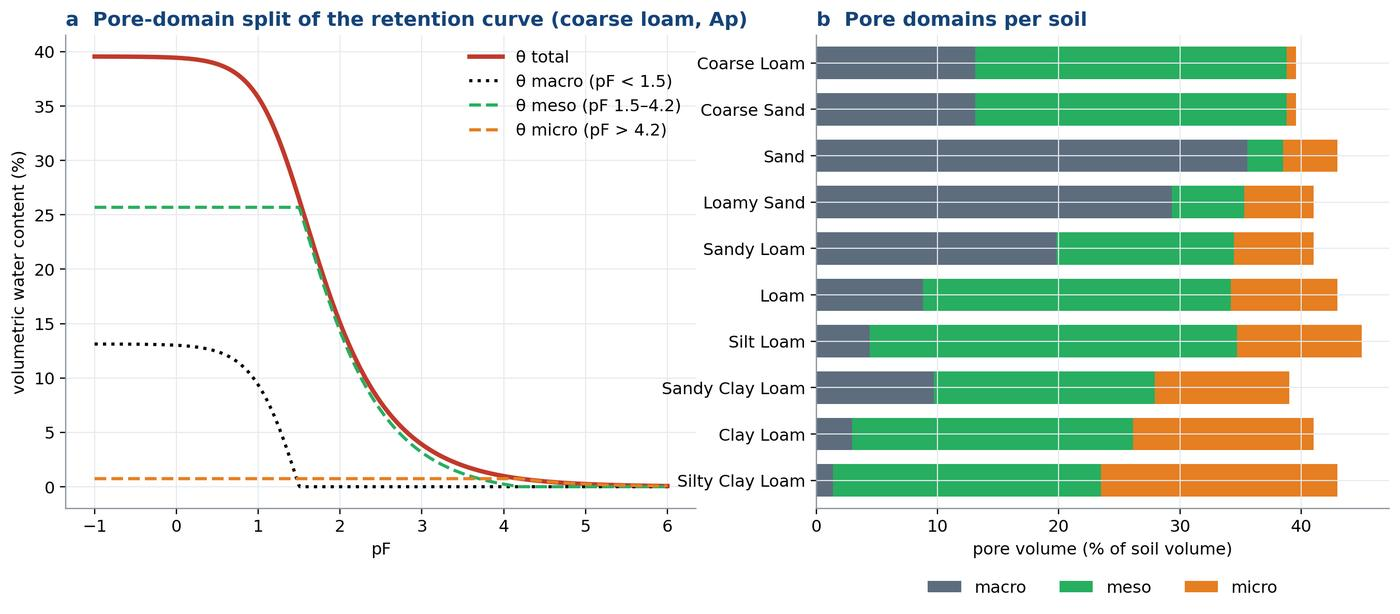
\includegraphics[width=0.84\textwidth]{fig/at/a21_02.jpg}}\caption{Pore-domain decomposition of the ten soils of the study from their retention curves (the same classes as Figure~\ref{fig:pg-dom}); the figure is described with its equation in Chapter~\ref{chap:21}.}\end{figure}

\banner{The flow in the pores: the law of Hagen and Poiseuille}
\section{Flow in one capillary tube}
The flow of a viscous fluid in a straight tube was measured by Hagen (1839) and Poiseuille (1840) and derived from the equations of fluid motion. Consider a laminar flow in a tube of radius $r$ and length $L$ under a pressure difference $\Delta p$. The velocity is zero at the wall and largest at the axis; its profile is a parabola, $v(\rho)=\Delta p\,(r^2-\rho^2)/(4\mu L)$ at the distance $\rho$ from the axis, where $\mu$ is the viscosity of the fluid. Integrating over the cross-section gives the volume flow rate
\begin{equation}\label{eq:pg-hp}\boxed{Q=\frac{\pi\,r^{4}\,\Delta p}{8\,\mu\,L}\ ,\qquad \bar v=\frac{Q}{\pi r^2}=\frac{r^{2}\,\Delta p}{8\,\mu\,L},}\end{equation}
where $Q$ is the flow (m$^3$\,s$^{-1}$), $\mu=1.0\times10^{-3}$ Pa\,s the dynamic viscosity of water at 20 $^\circ$C and $\bar v$ the mean velocity. For a vertical tube open to the air at both ends, $\Delta p/L=\rho_wg$ (a unit hydraulic gradient).
\par\noindent \textbf{Notes:} 1. The flow depends on the \emph{fourth power} of the radius: a tube twice as wide carries sixteen times as much water. 2. The law holds for laminar flow, which is the case when the Reynolds number $Re=\rho\bar v\,2r/\mu$ is below about 2000; in soil pores $Re$ is much smaller than 1. 3. The viscosity of water falls as the temperature rises (it is 1.0 mPa\,s at 20 $^\circ$C and 1.8 at 0 $^\circ$C), so that the conductivity of a soil rises by about 2 per cent per degree.

\exbox{The flow in one macropore}{A cylindrical pore of radius 0.5 mm, such as a worm channel, is full of water and drains under gravity (unit gradient). Find the mean velocity and the discharge.}\sol \givenline{$r=0.5\times10^{-3}$ m ; $\Delta p/L=\rho_wg=998\times9.81=9790$ Pa\,m$^{-1}$ ; $\mu=1.0\times10^{-3}$ Pa\,s}
\par\noindent From Equation~(\ref{eq:pg-hp}), $\bar v=\dfrac{r^2\,(\Delta p/L)}{8\mu}=\dfrac{(0.5\times10^{-3})^2\times9790}{8\times10^{-3}}=0.306$ m\,s$^{-1}$ \finans, about 30 cm per second, which is fast. The discharge is $Q=\pi r^2\bar v=\pi\times(0.5\times10^{-3})^2\times0.306=2.40\times10^{-7}$ m$^3$\,s$^{-1}$ $=0.24$ mL\,s$^{-1}$, or $865$ mL per hour \finans. One such channel can pass nearly a litre of water per hour. Remember that the law assumes a smooth tube full of water; a real burrow is rough and partly filled, so the figure is an upper limit.

\section{The bundle of capillaries and the conductivity}\label{sec:bundle}
A porous medium is now represented by a bundle of straight, parallel capillaries. Let there be $N$ pores of radius $r$ per unit area of cross-section; the porosity is $\phi=N\pi r^2$ (the fraction of the area that is open). The volume of water that crosses a unit area in a unit time under the gradient $i=\Delta p/(\rho_wgL)$ is $q=N\,Q=N\pi r^4\rho_wg\,i/(8\mu)$. By Darcy's law $q=K_s\,i$, so that the saturated conductivity of the bundle is
\begin{equation}\label{eq:pg-bundle}\boxed{K_s=\frac{\rho_w\,g}{8\,\mu}\,\phi\,r^{2}=\frac{\rho_w\,g}{\mu}\,k,\qquad k=\frac{\phi\,r^{2}}{8},}\end{equation}
where $k$ (m$^2$) is the \kw{intrinsic permeability} (a property of the pore geometry only), and $K_s$ the hydraulic conductivity (m\,s$^{-1}$), which includes the properties of the water. The result shows that the conductivity depends on the \emph{square} of the pore radius, and on the porosity only linearly: a tenfold reduction of the pore radius reduces the conductivity a hundredfold, while a tenfold reduction of the porosity reduces it tenfold. This is the reason why a clay with a porosity of 0.5 conducts much less than a sand with a porosity of 0.4.

\begin{figure}[!htbp]\centering\Lfig{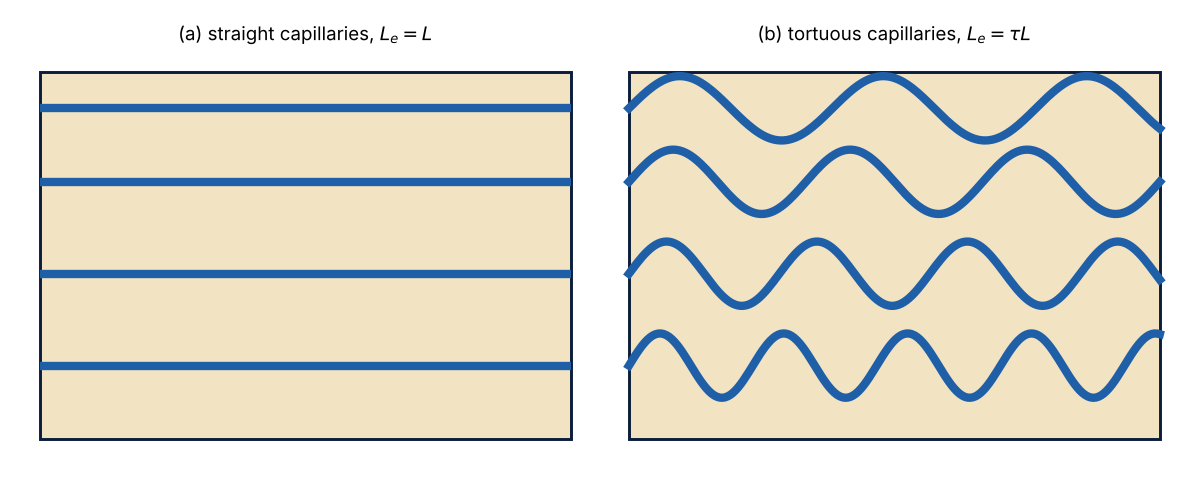
\includegraphics[width=0.84\textwidth]{fig/pore_tort.png}}\caption{(a) A bundle of straight parallel capillaries; (b) a bundle of tortuous capillaries, in which the water follows a path longer than the sample.}\end{figure}

\exbox{The conductivity of three bundles}{Find the saturated conductivity of a bundle of capillaries with porosity $\phi=0.40$ and radii $r=50\ \mu$m, $5\ \mu$m and $0.5\ \mu$m.}\sol \givenline{$\phi=0.40$ ; $r=50,\ 5,\ 0.5\ \mu$m ; $\rho_wg/(8\mu)=998\times9.81/(8\times10^{-3})=1.224\times10^{6}$ m$^{-1}$\,s$^{-1}$}
\par\noindent From Equation~(\ref{eq:pg-bundle}), $K_s=1.224\times10^6\times\phi\,r^2$.
\par\noindent For $r=50\times10^{-6}$ m: $K_s=1.224\times10^6\times0.40\times2.5\times10^{-9}=1.22\times10^{-3}$ m\,s$^{-1}$ $=1.06\times10^{4}$ cm\,d$^{-1}$ \finans.
\par\noindent For $r=5\ \mu$m: $K_s=1.22\times10^{-5}$ m\,s$^{-1}$ $=106$ cm\,d$^{-1}$ \finans.
\par\noindent For $r=0.5\ \mu$m: $K_s=1.22\times10^{-7}$ m\,s$^{-1}$ $=1.06$ cm\,d$^{-1}$ \finans.
\par\noindent Each tenfold reduction of the radius divides the conductivity by 100, so that the three bundles cover the range from a clean sand to a clay, although they have the same porosity. The values are larger than those measured on real soils of the same pore size, because a real pore is not straight, and the correction is the subject of the next sections.

\section{The distribution of the flow among the pores}
A real soil has pores of many sizes, and the flow is shared among them according to their sizes. If the pore volume in the radius class $r$ is $\mathrm d\phi(r)$, then the conductivity of the class is proportional to $r^2\,\mathrm d\phi$ (Equation~\ref{eq:pg-bundle}), so that the \emph{share of the flow} carried by the pores up to radius $r$ is
\begin{equation}\label{eq:pg-share}\boxed{\Phi_Q(r)=\frac{\int_0^{r}r'^{2}\,\mathrm d\phi(r')}{\int_0^{\infty}r'^{2}\,\mathrm d\phi(r')}\ ,}\end{equation}
which is smaller than the share of the pore volume $\Phi_V(r)=\phi(r)/\phi$ for all $r$, because the large pores weigh more in the flow. Figure~\ref{fig:pg-flux} shows the result for a soil in which the pore volume is distributed log-normally around a median radius of 10 $\mu$m: half of the pore volume lies in pores narrower than 10 $\mu$m, yet these carry only about 3 per cent of the flow, and the pores wider than 50 $\mu$m, which are about 5 per cent of the volume, carry more than half of it.
\begin{figure}[!htbp]\centering\Lfig{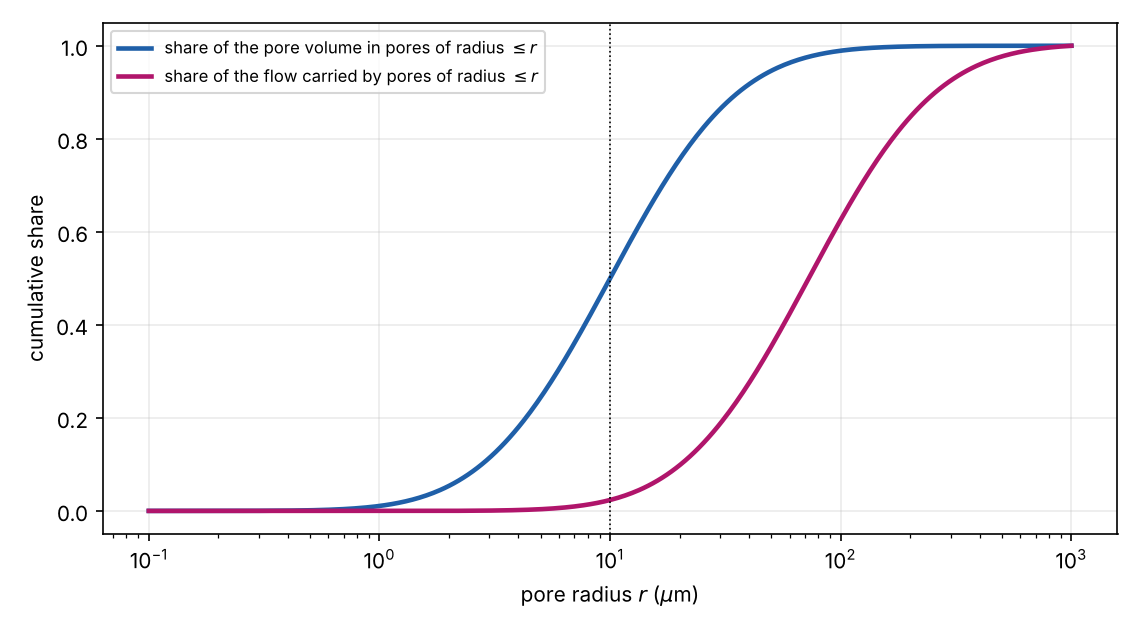
\includegraphics[width=0.84\textwidth]{fig/pore_flux.png}}\caption{The cumulative share of the pore volume (blue) and of the saturated flow (magenta) as a function of the pore radius, for a log-normal pore-size distribution with a median radius of 10 $\mu$m and a standard deviation of the logarithm of 1.0.}\label{fig:pg-flux}\end{figure}
\par\noindent This distribution has an important consequence for the unsaturated soil. As the soil dries, the largest pores empty first, and with them the largest part of the conductivity: when the suction rises to 100 cm (the field capacity), all pores wider than 15 $\mu$m are empty and the conductivity has fallen by one or two orders of magnitude although more than half of the water is still there. This is the geometric reason for the curve of the conductivity in Chapter~\ref{chap:01} and for the failure of a dry soil to supply a root.

\exbox{How many small pores equal one large pore?}{How many pores of radius 10 $\mu$m are needed to carry the same flow as one earthworm channel of radius 2 mm, under the same gradient?}\sol \givenline{$r_1=2000\ \mu$m ; $r_2=10\ \mu$m ; same $\Delta p/L$}
\par\noindent From Equation~(\ref{eq:pg-hp}), the flow of a tube is proportional to $r^4$, so the number of small tubes is $N=(r_1/r_2)^4=(2000/10)^4=200^4=1.6\times10^{9}$ \finans. It takes 1.6 thousand million small pores to carry the water of one worm channel. A square metre of soil of porosity 0.3 that consisted of nothing but pores of radius 10 $\mu$m would hold $N=\phi/(\pi r^2)=0.3/(\pi\times10^{-10})=9.5\times10^{8}$ of them: fewer than the number needed to replace one worm channel. This explains why a few biopores, in a soil in which the matrix is slow, determine the rate at which the soil takes water in a heavy rain.

\banner{Tortuosity, connection and the real conductivity}
\section{Tortuosity}
The pores of a soil are not straight. The water follows a winding path whose length $L_e$ is longer than the straight distance $L$ between the ends. The ratio
\begin{equation}\label{eq:pg-tort}\boxed{\tau=\frac{L_e}{L}\ \ (\geq1)}\end{equation}
is the \kw{tortuosity} (some authors use $\tau$ for the inverse, or its square; the definition must be checked). The effect is double: the path is longer (so the gradient along the path is $\Delta p/L_e$, smaller than $\Delta p/L$) and the actual velocity is directed along the path, so that its component along the sample is reduced again. For a bundle of tortuous capillaries the conductivity of Equation~(\ref{eq:pg-bundle}) is divided by $\tau^2$:
\[K_s=\frac{\rho_wg}{8\mu}\,\frac{\phi\,r^2}{\tau^2}.\]
Typical values for $\tau$ are 1.2 to 1.6 for sands, and 2 to 5 for aggregated soils and clays. The same factor applies to diffusion: the gas and solute diffusion coefficients in a soil are smaller than those of free water or air by $\phi/\tau^2$.

\exbox{The effect of tortuosity}{Correct the conductivity of the bundle with $r=50\ \mu$m and $\phi=0.40$ found in the earlier example for a tortuosity of $\tau=1.5$.}\sol \givenline{$K_s=1.06\times10^4$ cm\,d$^{-1}$ ; $\tau=1.5$}
\par\noindent $K_s=1.06\times10^4/1.5^2=1.06\times10^4/2.25=4.70\times10^3$ cm\,d$^{-1}$ \finans. A tortuosity of 1.5, which is only a modest bending of the path, halves the conductivity.

\section{Connection of the pores: bodies and throats}
A pore in a soil has a wide part (the \kw{body}) and a narrow passage to the next pore (the \kw{throat}). The flow is limited by the throats, and the retention (the emptying) is also limited by the throats during drying, but by the bodies during wetting. Thus a pore that is large but connected only through narrow throats behaves, for the flow, like a narrow pore: this is the cause of the hysteresis and of the fact that a conductivity calculated from the pore sizes of the retention curve is too high unless a connection factor is applied. The factor $\ell$ in the conductivity function of Mualem (Chapter~\ref{chap:01}) is such a connection and tortuosity factor, with a value of about $0.5$ for most soils.
\par\noindent \textbf{Note:} If the pores were connected at random, there would exist a \kw{percolation threshold}: a minimum fraction of the pore space that must be open to form a path across the sample (about 0.3 in three dimensions for a random network). A soil whose air-filled porosity falls below this value, as in a waterlogged soil, loses the continuity of the gas phase, and the oxygen cannot move.

\begin{figure}[!htbp]\centering\Lfig{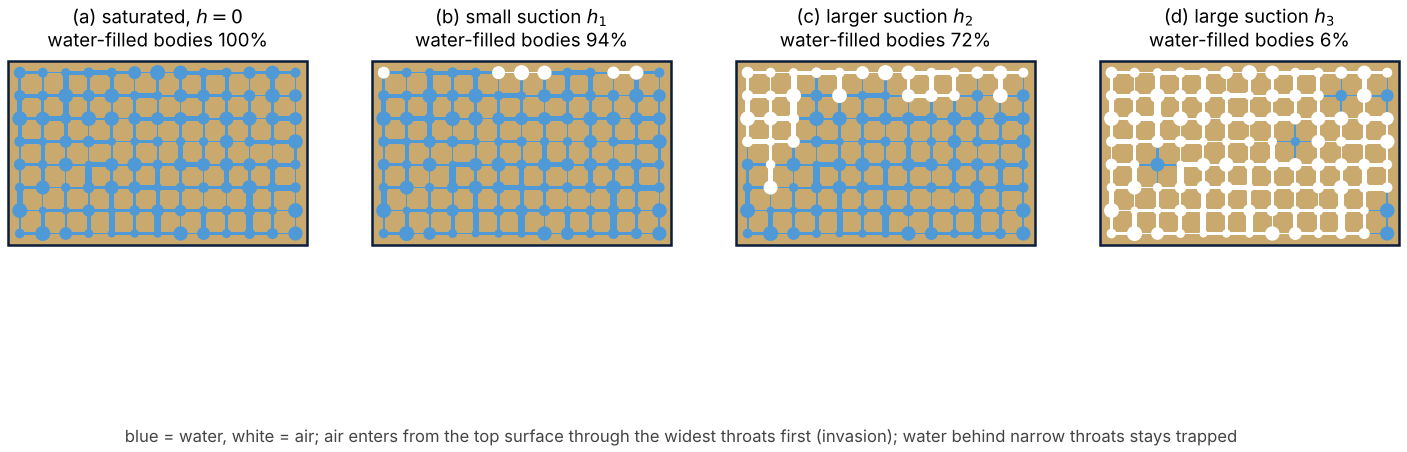
\includegraphics[width=0.92\textwidth]{fig/pg_network.png}}\caption{Drying of a network of pore bodies and throats, from (a) saturated to (d) a large suction. The large bodies empty first, but only when a throat that connects them to the air has emptied; the flow is limited by the narrowest throat on the path, and the water that is left is held in the smallest pores.}\end{figure}

\section{The specific surface and the hydraulic radius}
The \kw{specific surface} is the area of the walls of the pores per unit volume of solid. For spheres of diameter $d$, $S_0=6/d$ (m$^{-1}$). Fine grains have an enormous surface: 1 cm$^3$ of sand of $d=0.5$ mm has an area of $120$ cm$^2$, whereas 1 cm$^3$ of clay with plates of 1 $\mu$m has $6\times10^{4}$ cm$^2$ or more, and a swelling clay such as montmorillonite has an internal surface of up to 800 m$^2$ per gram. The surface determines how much water is held as films, the adsorption of ions and the heat of wetting. The \kw{hydraulic radius} of a pore space is the ratio of its volume to its wall area,
\[ m_h=\frac{\phi}{S_0(1-\phi)},\]
which for a cylinder of radius $r$ is $r/2$. It is the length that replaces the radius of a capillary in a medium of irregular pores.

\section{The Kozeny--Carman equation}
Kozeny (1927) and Carman (1937) used the hydraulic radius and the tortuosity to derive a conductivity from the grain size and the porosity, without any assumption about the shape of the pores. The result for the permeability and the conductivity is
\begin{equation}\label{eq:pg-kc}\boxed{k=\frac{\phi^{3}}{c_{KC}\,S_0^{2}\,(1-\phi)^{2}},\qquad K_s=\frac{\rho_wg}{\mu}\,k,}\end{equation}
where $c_{KC}\approx5$ is the Kozeny constant (it contains the shape factor and the tortuosity), and $S_0=6/d_e$ for grains with an effective diameter $d_e$. The strong dependence of the conductivity on the porosity, as $\phi^3/(1-\phi)^2$, shows that a small change of the porosity gives a large change in the conductivity: a decrease of $\phi$ from 0.40 to 0.35 reduces $K_s$ by a factor of $(0.35/0.40)^3\,(0.60/0.65)^2=0.57$.

\exbox{The conductivity of a sand and of a silt from the grain size}{Use the Kozeny--Carman equation to find the saturated conductivity of (a) a sand of effective grain diameter $d=0.5$ mm and (b) a silt of $d=0.05$ mm. Take $\phi=0.40$ and $c_{KC}=5$.}\sol \givenline{$\phi=0.40$ ; $c_{KC}=5$ ; (a) $d=0.5$ mm ; (b) $d=0.05$ mm ; $\rho_wg/\mu=9.79\times10^{6}$ m$^{-1}$\,s$^{-1}$}
\par\noindent \textbf{(a)} $S_0=6/d=6/(0.5\times10^{-3})=1.2\times10^{4}$ m$^{-1}$. The permeability is
\[k=\frac{0.40^3}{5\times(1.2\times10^4)^2\times0.60^2}=\frac{0.064}{2.592\times10^{8}}=2.47\times10^{-10}\ \text{m}^2.\]
Then $K_s=9.79\times10^{6}\times2.47\times10^{-10}=2.42\times10^{-3}$ m\,s$^{-1}$ $=2.1\times10^{4}$ cm\,d$^{-1}$ \finans, the order of magnitude of a clean medium sand.
\par\noindent \textbf{(b)} The diameter is ten times smaller, $S_0$ ten times larger, so $k$ is a hundred times smaller: $K_s=209$ cm\,d$^{-1}$ \finans. The silt of ideal spheres still has a high conductivity because it has no aggregates and no clay; real silts have a lower value, since the grains are not equal and the flow paths are narrower.

\banner{Models of the pore-size distribution}
\section{Power-law and log-normal models}
The retention curve is measured at a few suctions and must be described by a function. Three families are in use, and each makes a different assumption about the distribution of the pores.
\begin{exlist}
\item \kw{Brooks and Corey (1964).} The effective saturation falls as a power of the suction beyond an \emph{air-entry} value $h_b$:
\begin{equation}\label{eq:pg-bc}\boxed{S_e=\Bigl(\frac{h_b}{h}\Bigr)^{\lambda}\ (h>h_b),\qquad K=K_s\,S_e^{\,(2+3\lambda)/\lambda}}\end{equation}
where $\lambda$ is the \emph{pore-size index} (large for a narrow distribution, as in a uniform sand, $\lambda\approx2$ to $4$, and small for a wide distribution, as in a clay, $\lambda\approx0.1$ to $0.3$) and the conductivity follows from the model of Burdine. The power law is a good description of a soil with a clear air-entry suction, and it implies that the pore volume has a fractal (self-similar) distribution.
\item \kw{van Genuchten (1980).} A smooth curve with no air-entry value (Chapter~\ref{chap:01}), which has become the standard in Daisy and in this book, because it describes the curvature near saturation that the power law lacks, and its conductivity has a closed form.
\item \kw{Kosugi (1996).} The pore radii are assumed to follow a log-normal distribution, so that the retention curve is the complementary cumulative normal distribution of $\ln h$, with the median pore size and the standard deviation of the logarithm as parameters. It has a direct geometric meaning.
\end{exlist}

\exbox{The conductivity of a Brooks--Corey soil}{A soil has a pore-size index $\lambda=0.5$ and a saturated conductivity $K_s=10$ cm\,d$^{-1}$. Find its conductivity at an effective saturation $S_e=0.30$ and the ratio to $K_s$.}\sol \givenline{$\lambda=0.5$ ; $K_s=10$ cm\,d$^{-1}$ ; $S_e=0.30$}
\par\noindent The exponent is $(2+3\lambda)/\lambda=(2+1.5)/0.5=7$. From Equation~(\ref{eq:pg-bc}), $K/K_s=0.30^7=2.19\times10^{-4}$ \finans, so $K=10\times2.19\times10^{-4}=2.2\times10^{-3}$ cm\,d$^{-1}$ \finans. The soil has lost 99.98 per cent of its conductivity when it has lost 70 per cent of its effective water: the large pores that carry the flow are the first to empty.

\section{The pores of aggregates: dual porosity}
In a structured soil the pore space has two parts that behave differently: the \kw{matrix} (the pores inside the aggregates, small and well connected, in which the water is held strongly) and the \kw{macropores} between the aggregates and the biopores (large, with a different flow). In a \kw{dual-porosity} model each domain has its own retention curve and conductivity, and a transfer term between them; in Daisy the biopores are added to the matrix as a second system that takes the water above a given rate, and passes it to the drains. A soil with a dual porosity has a retention curve with \emph{two steps} (a large one at small suction for the inter-aggregate pores and a second one at large suction for the intra-aggregate pores), and a conductivity curve with a sudden drop near saturation.

\section{Flow in cracks and macropores: the cubic law}
A crack with parallel smooth walls and an aperture $b$ is the simplest model of a shrinkage crack. Integrating the equation of motion between two plates gives the flow per unit width of crack,
\begin{equation}\label{eq:pg-crack}\boxed{q_c=\frac{\rho_w\,g\,b^{3}}{12\,\mu}\,i,}\end{equation}
where $q_c$ is in m$^2$\,s$^{-1}$ and $i$ is the hydraulic gradient: the flow depends on the \emph{cube} of the aperture (the cubic law). A crack of 0.2 mm width and 1 m length, drained under unit gradient, carries $q_c=998\times9.81\times(2\times10^{-4})^3/(12\times10^{-3})=6.5\times10^{-6}$ m$^2$\,s$^{-1}$, which is 23 L per hour per metre of crack \finans, many times what the matrix carries over the same width. When the clay is wetted, the crack closes by swelling and the flow stops.

\banner{Changes of the geometry: tillage, compaction and life}
\section{How management and life change the pore space}
The geometry of the pores is not a fixed property. It is made and unmade every year. \kw{Tillage} loosens the topsoil and raises the macroporosity for a few weeks, but also breaks the continuity of the biopores and lowers the stability of the aggregates, so that after some rains the surface settles and may seal (see the \emph{consolidation} of Chapter~\ref{chap:10}). \kw{Compaction} by heavy machines destroys the macropores first, as the example of this chapter shows, and with them the aeration and the rate of drainage. \kw{Roots} make biopores when they die and decay, and the exudates of living roots bind the aggregates. \kw{Worms} burrow and cast, producing a network of channels that stays open for years under no-till. \kw{Wetting and drying}, and \kw{freezing and thawing}, open and close cracks in clay soils.
\par\noindent In this book the effect is represented by a single number, the \kw{pore index} of the structure, which scales the macropore part of the retention curve and the saturated conductivity (Chapter~\ref{chap:10}); the workbench shows the section of a modelled topsoil with the pore classes coloured (Chapter~\ref{chap:08}).

\section{Measuring the geometry of the pores}
Four groups of methods are used.
\begin{exlist}
\item \kw{The retention curve.} The measurement of $\theta$ at several suctions gives the distribution of the pore sizes by Equation~(\ref{eq:pg-psd}); it is the method of this book, because the data are available for every soil.
\item \kw{Mercury intrusion porosimetry.} Mercury does not wet the soil, so it must be forced into the pores by pressure $P$. The radius entered at the pressure $P$ follows the equation of Washburn, $r=-2\gamma_{Hg}\cos\beta_{Hg}/P$ with $\gamma_{Hg}=0.485$ N\,m$^{-1}$ and $\beta_{Hg}=140^\circ$, which gives $r=7.4\ \mu$m at 1 bar and $0.074\ \mu$m at 100 bar. It measures pore \emph{throats}, and the pressure may damage the structure.
\item \kw{Gas adsorption.} The amount of nitrogen gas adsorbed at different pressures gives the specific surface (the equation of Brunauer, Emmett and Teller, BET) and the micropores below 0.1 $\mu$m.
\item \kw{Imaging.} A thin section of the soil impregnated with resin is examined under the microscope; X-ray computed tomography scans a core non-destructively at a resolution of 5 to 50 $\mu$m, and the images are analysed for the volume, the connection and the shape of the pores (Chapter~\ref{chap:11} treats the volumetric scan). The \kw{Euler number}, which counts the number of the independent loops of a pore network, is a measure of its connection.
\end{exlist}
\noindent \textbf{Note:} Each method sees a different part of the pore space, and the results cannot be compared without care: the retention curve gives the \emph{necks} that empty, the images show the \emph{bodies} that the resolution allows, and the mercury intrusion shows the \emph{throats} accessible from the surface.

\section{Summary of the geometry}
\begin{itemize}
\item The pores are classified by their origin (textural, structural, biopores), by size (macro, meso, micro) and by function (transmission, storage, residual).
\item The suction at which a pore empties is inversely proportional to its radius (Equation~\ref{eq:pg-cap}); the retention curve is therefore the pore-size distribution.
\item The flow in a pore is proportional to the fourth power of its radius and the conductivity of a bundle to the square (Equations~\ref{eq:pg-hp} and~\ref{eq:pg-bundle}); a few large pores carry most of the flow.
\item The tortuosity and the connection of the pores lower the conductivity (Equations~\ref{eq:pg-tort} and~\ref{eq:pg-kc}); a model must include them.
\item The geometry changes with tillage, compaction, roots, worms and drying; macropores change first and most.
\end{itemize}

\backhead{EXERCISES}{khred}
\begin{exlist}
\item A soil has $\rho_b=1.45$ g\,cm$^{-3}$ and $\rho_s=2.65$ g\,cm$^{-3}$. Find the porosity. \exans{0.453}
\item What is the capillary rise in a pore of radius 20 $\mu$m? \exans{74.5 cm}
\item What is the radius of the largest water-filled pore at pF 3? \exans{1.49 $\mu$m}
\item A tube has a radius four times that of another. By what factor is its Poiseuille flow larger, for the same gradient? \exans{256}
\item Find the conductivity of a bundle of capillaries with $r=20\ \mu$m and $\phi=0.35$ (no tortuosity). \exans{1.48$\times10^3$ cm/d}
\item Find the Kozeny--Carman conductivity for $d=0.1$ mm, $\phi=0.40$, $c_{KC}=5$. \exans{835 cm/d}
\item For a Brooks--Corey soil with $\lambda=0.4$, find $K/K_s$ at $S_e=0.5$. \exans{3.9$\times10^{-3}$}
\item What is the radius entered by mercury at a pressure of 10 bar? \exans{0.74 $\mu$m}
\item Find the flow per metre of a crack of 0.2 mm aperture under unit gradient, in litres per hour. \exans{23.5 L/h}
\item A soil is compacted from $\rho_b=1.30$ to $1.50$ g\,cm$^{-3}$ ($\rho_s=2.65$). How much porosity is lost? \exans{0.075}
\end{exlist}

\dykband{DO YOU KNOW ?}
\begin{exlist}
\item What is the difference between a textural and a structural pore?
\item Why does a narrow pore hold water at a higher suction than a wide one?
\item State the law of Young and Laplace, and say what is meant by the contact angle.
\item Why does the flow in a tube depend on the fourth power of its radius, and the conductivity of a bundle on the square?
\item What is tortuosity, and how does it change the conductivity?
\item What is the difference between the body and the throat of a pore, and which controls the emptying?
\item Why are a few biopores more important for infiltration than millions of small pores?
\item How does a heavy tractor change the geometry of the pores?
\end{exlist}

\backhead{OBJECTIVE TYPE QUESTIONS}{khred}
\begin{exlist}
\item The suction at which a pore empties is
\opt{proportional to its radius}{inversely proportional to its radius}{independent of its radius}{proportional to its volume}
\item The flow in a cylindrical pore of radius $r$ is proportional to
\opt{$r$}{$r^{2}$}{$r^{3}$}{$r^{4}$}
\item The conductivity of a bundle of capillaries of equal radius is proportional to
\opt{$r$}{$r^{2}$}{$r^{3}$}{$r^{4}$}
\item The pores that are emptied at suctions below 100 cm are called
\opt{micropores}{mesopores}{macropores}{residual pores}
\item Tortuosity is the ratio of
\opt{the path length to the sample length}{the porosity to the density}{the pore radius to the grain radius}{the throat to the body}
\item The flow in a crack of aperture $b$ is proportional to
\opt{$b$}{$b^{2}$}{$b^{3}$}{$b^{4}$}
\end{exlist}
\objkey{1.\ (b),\quad 2.\ (d),\quad 3.\ (b),\quad 4.\ (c),\quad 5.\ (a),\quad 6.\ (c)}
\swaflvideo{23}
